\documentclass[12pt]{book}
\usepackage[spanish]{babel}
\usepackage[utf8]{inputenc}

\usepackage{graphicx,subfigure}
\usepackage{wrapfig, blindtext}
\usepackage{listings}
\usepackage{xcolor}
\usepackage{bookman}
\usepackage[document]{ragged2e}
\setcounter{section}{+1}
\setcounter{figure}{-1}
% \ltset{
% 	backgroundcolor=\color{black!5},
% 	basicstyle=\footnotesize\ttfamily\small,
% }

\makeatletter
\renewcommand{\@makechapterhead}[1]{%
\vspace*{50 pt}%
{\setlength{\parindent}{0pt} \raggedright \normalfont
\bfseries\Huge
\ifnum \value{secnumdepth}>1 
    \if@mainmatter\thechapter.\ \fi%
\fi
#1\par\nobreak\vspace{40 pt}}}
\makeatother

\graphicspath{ {img/} }

\title{\textbf{Catharina van Hemessen}}
\author{Alberto Navalón Lillo, 3ESO A}

\begin{document}

\frontmatter
\maketitle
\tableofcontents
\mainmatter

\addcontentsline{toc}{chapter}{Introducción}

% Introduction chapter
\chapter*{Introducción}
\chaptermark{Introducción}

En este trabajo de investigación se van a tratar la vida y obras de la pintora flamenca renacentista Catharina van Hemessen (1528?-1587?), quien es reconocida como la primera pintora flamenca de la cual se conserva una obra extensa y, además, de autenticidad verificada. Principalmente se la conoce por series de pequeños retratos femeninos datados de entre finales de la década de 1540 y principios de la década de 1550.\bigskip


A van Hemessen se la distingue por haber creado el primer autorretrato femenino conocido, su \textit{Autorretrato} (figura 0), datado en 1548, además por la propia autora, que escribió las siguientes palabras sobre el lienzo:\bigskip

\indent``\textit{Yo, Catharina van Hemessen, me he retratado a mí misma} / \textit{1548} / \textit{Ella de 20 años de edad}''\footnote{Del original: ``\textit{Ego Catarina de / Hemessen me / pinxi \textbf{1548} // Etatis suae / 20}''}\bigskip

Este retrato muestra a la artista en las fases tempranas de la creación de un retrato. En la actualidad, la obra pertenece a la colección del Kunstmuseum Basel, al que pertenece la mayor y más significativa colección pública de arte en Suiza. También podemos encontrar obras de van Hemessen en el Rijksmuseum de Ámsterdam y en la National Gallery de Londres.\bigskip

Como Catharina, muchas otras mujeres de su tiempo soñaban con ser pintoras y artistas. Sin embargo, no era un sueño fácil de conseguir para ellas, dado que su educación artística implicaría, entre otras cosas, la disección de cadáveres humanos y el estudio de la figura del cuerpo del hombre, lo que constituía una educación poco accesible a las mujeres, además de no muy placentera. Todo esto en adición a la discriminación hacia ellas, quienes eran consideradas incapaces de trabajar como artistas.\bigskip

\begin{wrapfigure}{l}{0.4\textwidth}
	\begin{center}
		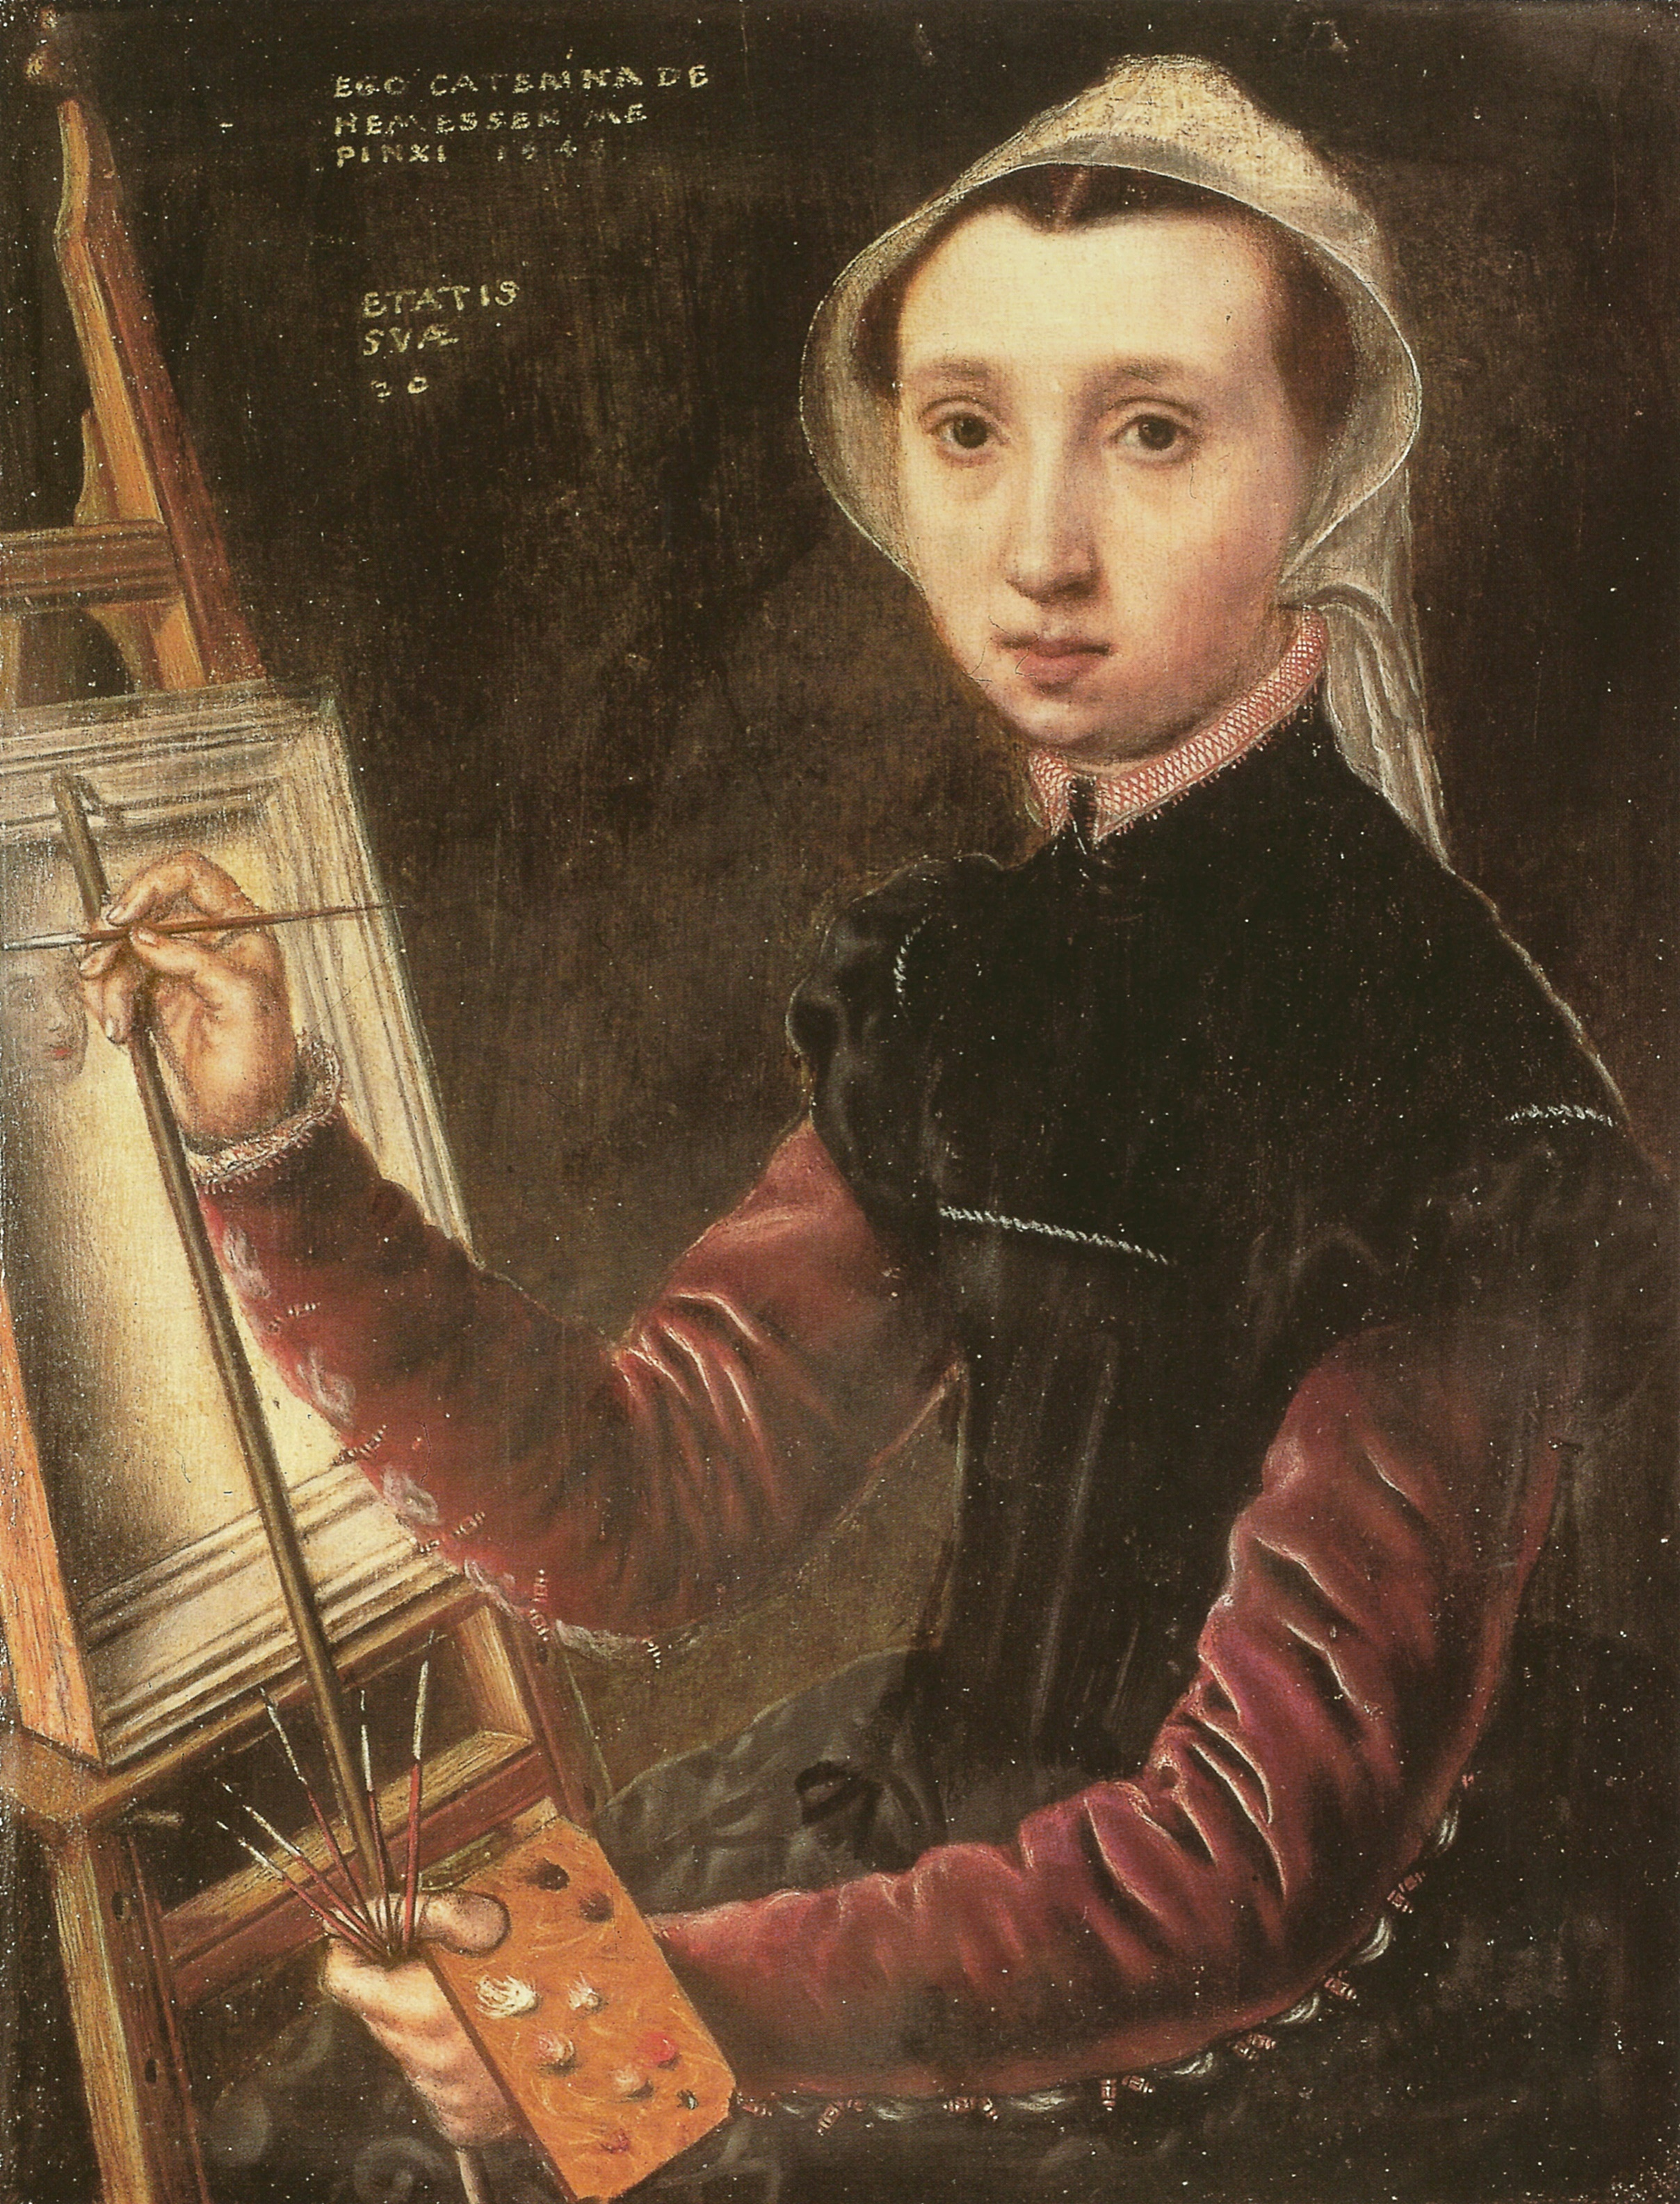
\includegraphics[width=0.9\linewidth]{self-portrait}
		\caption{\textit{Autorretrato}, Catharina van Hemessen, 1548}
		\label{fig:wrapfig}
	\end{center}
\end{wrapfigure}

En adición a esto, el período de aprendizaje de los artistas en esta época también consistía en vivir durante cuatro o cinco años junto a un artista más veterano, quien le pudiese enseñar de primera mano. Por ello, pocas llegaban a esto, puesto que muy pocos artistas veteranos aceptarían en aquel entonces a una mujer como aprendiz; y las que realmente conseguían recibir esta educación, como es el caso de van Hemessen, lo hacían de parte de alguien cercano a ellos. Catharina fue instruida por su propio padre, Jan Sanders van Hemessen, un reputado pintor.\bigskip

Actualmente se ha identificado un total de 10 obras firmadas y datadas por la propia artista, entre las que se encuentran seis retratos, un autorretrato (su \textit{Autorretrato}), y pinturas religiosas en las que se muestran grandes grupos de figuras. Un ejemplo de su obra religiosa es su \textit{Cristo se encuentra con Verónica} (1541-1560), en que se representa la imagen bíblica de la Santa Faz.

% Biography
\chapter{Biografía}

Catharina van Hemessen nació en Amberes (Bélgica), muy probablemente en el año 1528, hija de Bárbara de Fevre, quien a su vez fue hija de un rico comerciante de la ciudad; y del pintor manierista y alumno del gran pintor y grabador flamenco Hendrick van Cleve, Jan Sanders Van Hemessen (Hemiksen, 1500?-Haarlem, 1566?). De este fue, presumiblemente, además de hija, aprendiz y discípula, y supuestamente colaboró con él en muchas de sus obras, como era costumbre en muchas mujeres artistas de la época. Formó parte del círculo de la corte hacia 1540, cuando entró junto a su padre, bajo el patronazgo de la reina María de Hungría (figura 1.1), de quien fue dama de honor.\bigskip

\begin{wrapfigure}{r}{0.4\textwidth}
	\begin{center}
		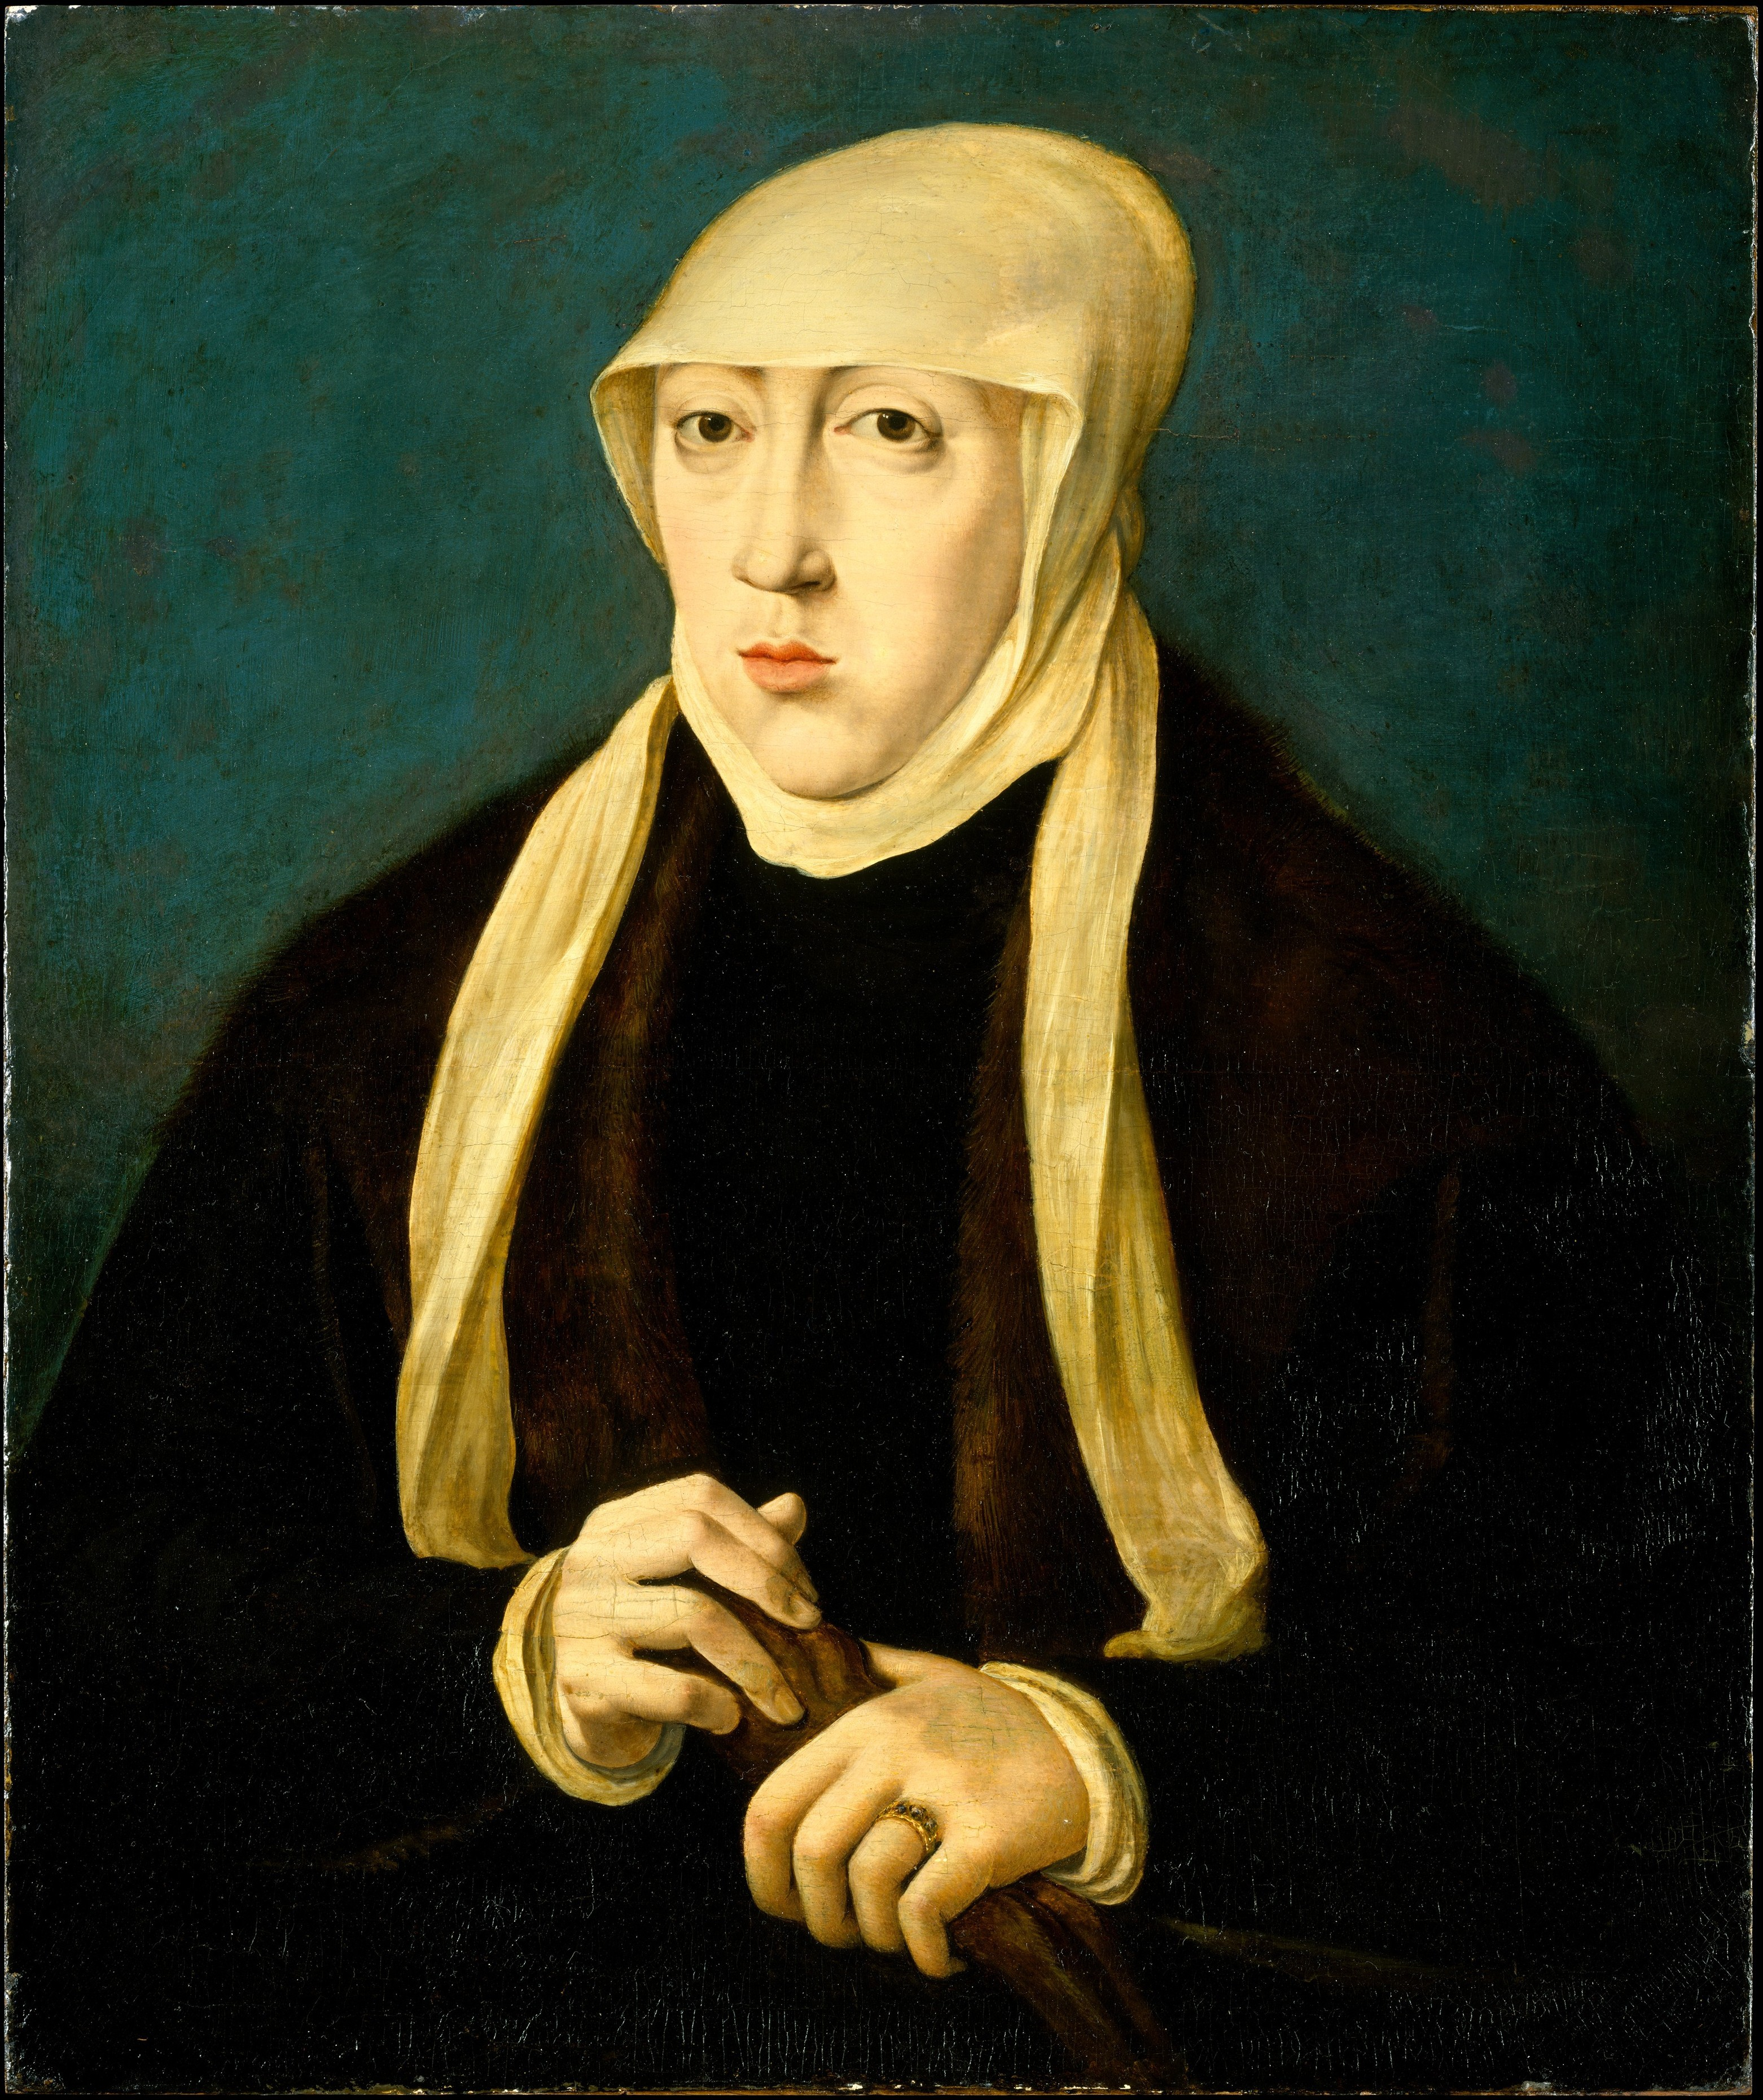
\includegraphics[width=0.9\linewidth]{mary-queen-of-hungary}
		\caption{María de Hungría, Habsburgo y Austria (1505-1558)}
		\label{fig:wrapfig}
	\end{center}
\end{wrapfigure}

En 1554, con aproximadamente 26 años, contrae matrimonio con Chrétien de Morien, el organista de la catedral de Amberes, cargo considerado importante en aquella época. A consecuencia de esto, su carrera artística se frena, seguramente para dedicarse exclusivamente a su matrimonio, dado que no se han hallado trabajos suyos datados a partir de esa época, con una única excepción de la que se tiene constancia, que será explicada a continuación.\bigskip

Sin embargo, cuando poco tiempo después María de Hungría renunció a la regencia y se marchó a vivir a España, Catharina y su marido se marcharon con ella, y disfrutaron de una vida más o menos acomodada gracias a la ayuda económica de la hermana del emperador.\bigskip

En el poco tiempo que la pareja quedó en España, es sabido que van Hemessen volvió a coger el pincel para colaborar en la creación del retablo de Tendilla del Monasterio Jerónimo de Santa Ana de Guadalajara. Tras analizar las pinturas del retablo se dedujo que fueron obra de cuatro pintores, además de Catharina, del taller de Jan Sanders van Hemessen. En 1915, tras su reaparición, fue adquirido por el Cincinnati Art Museum (EEUU).\bigskip

\begin{figure}[h]
	\centering
	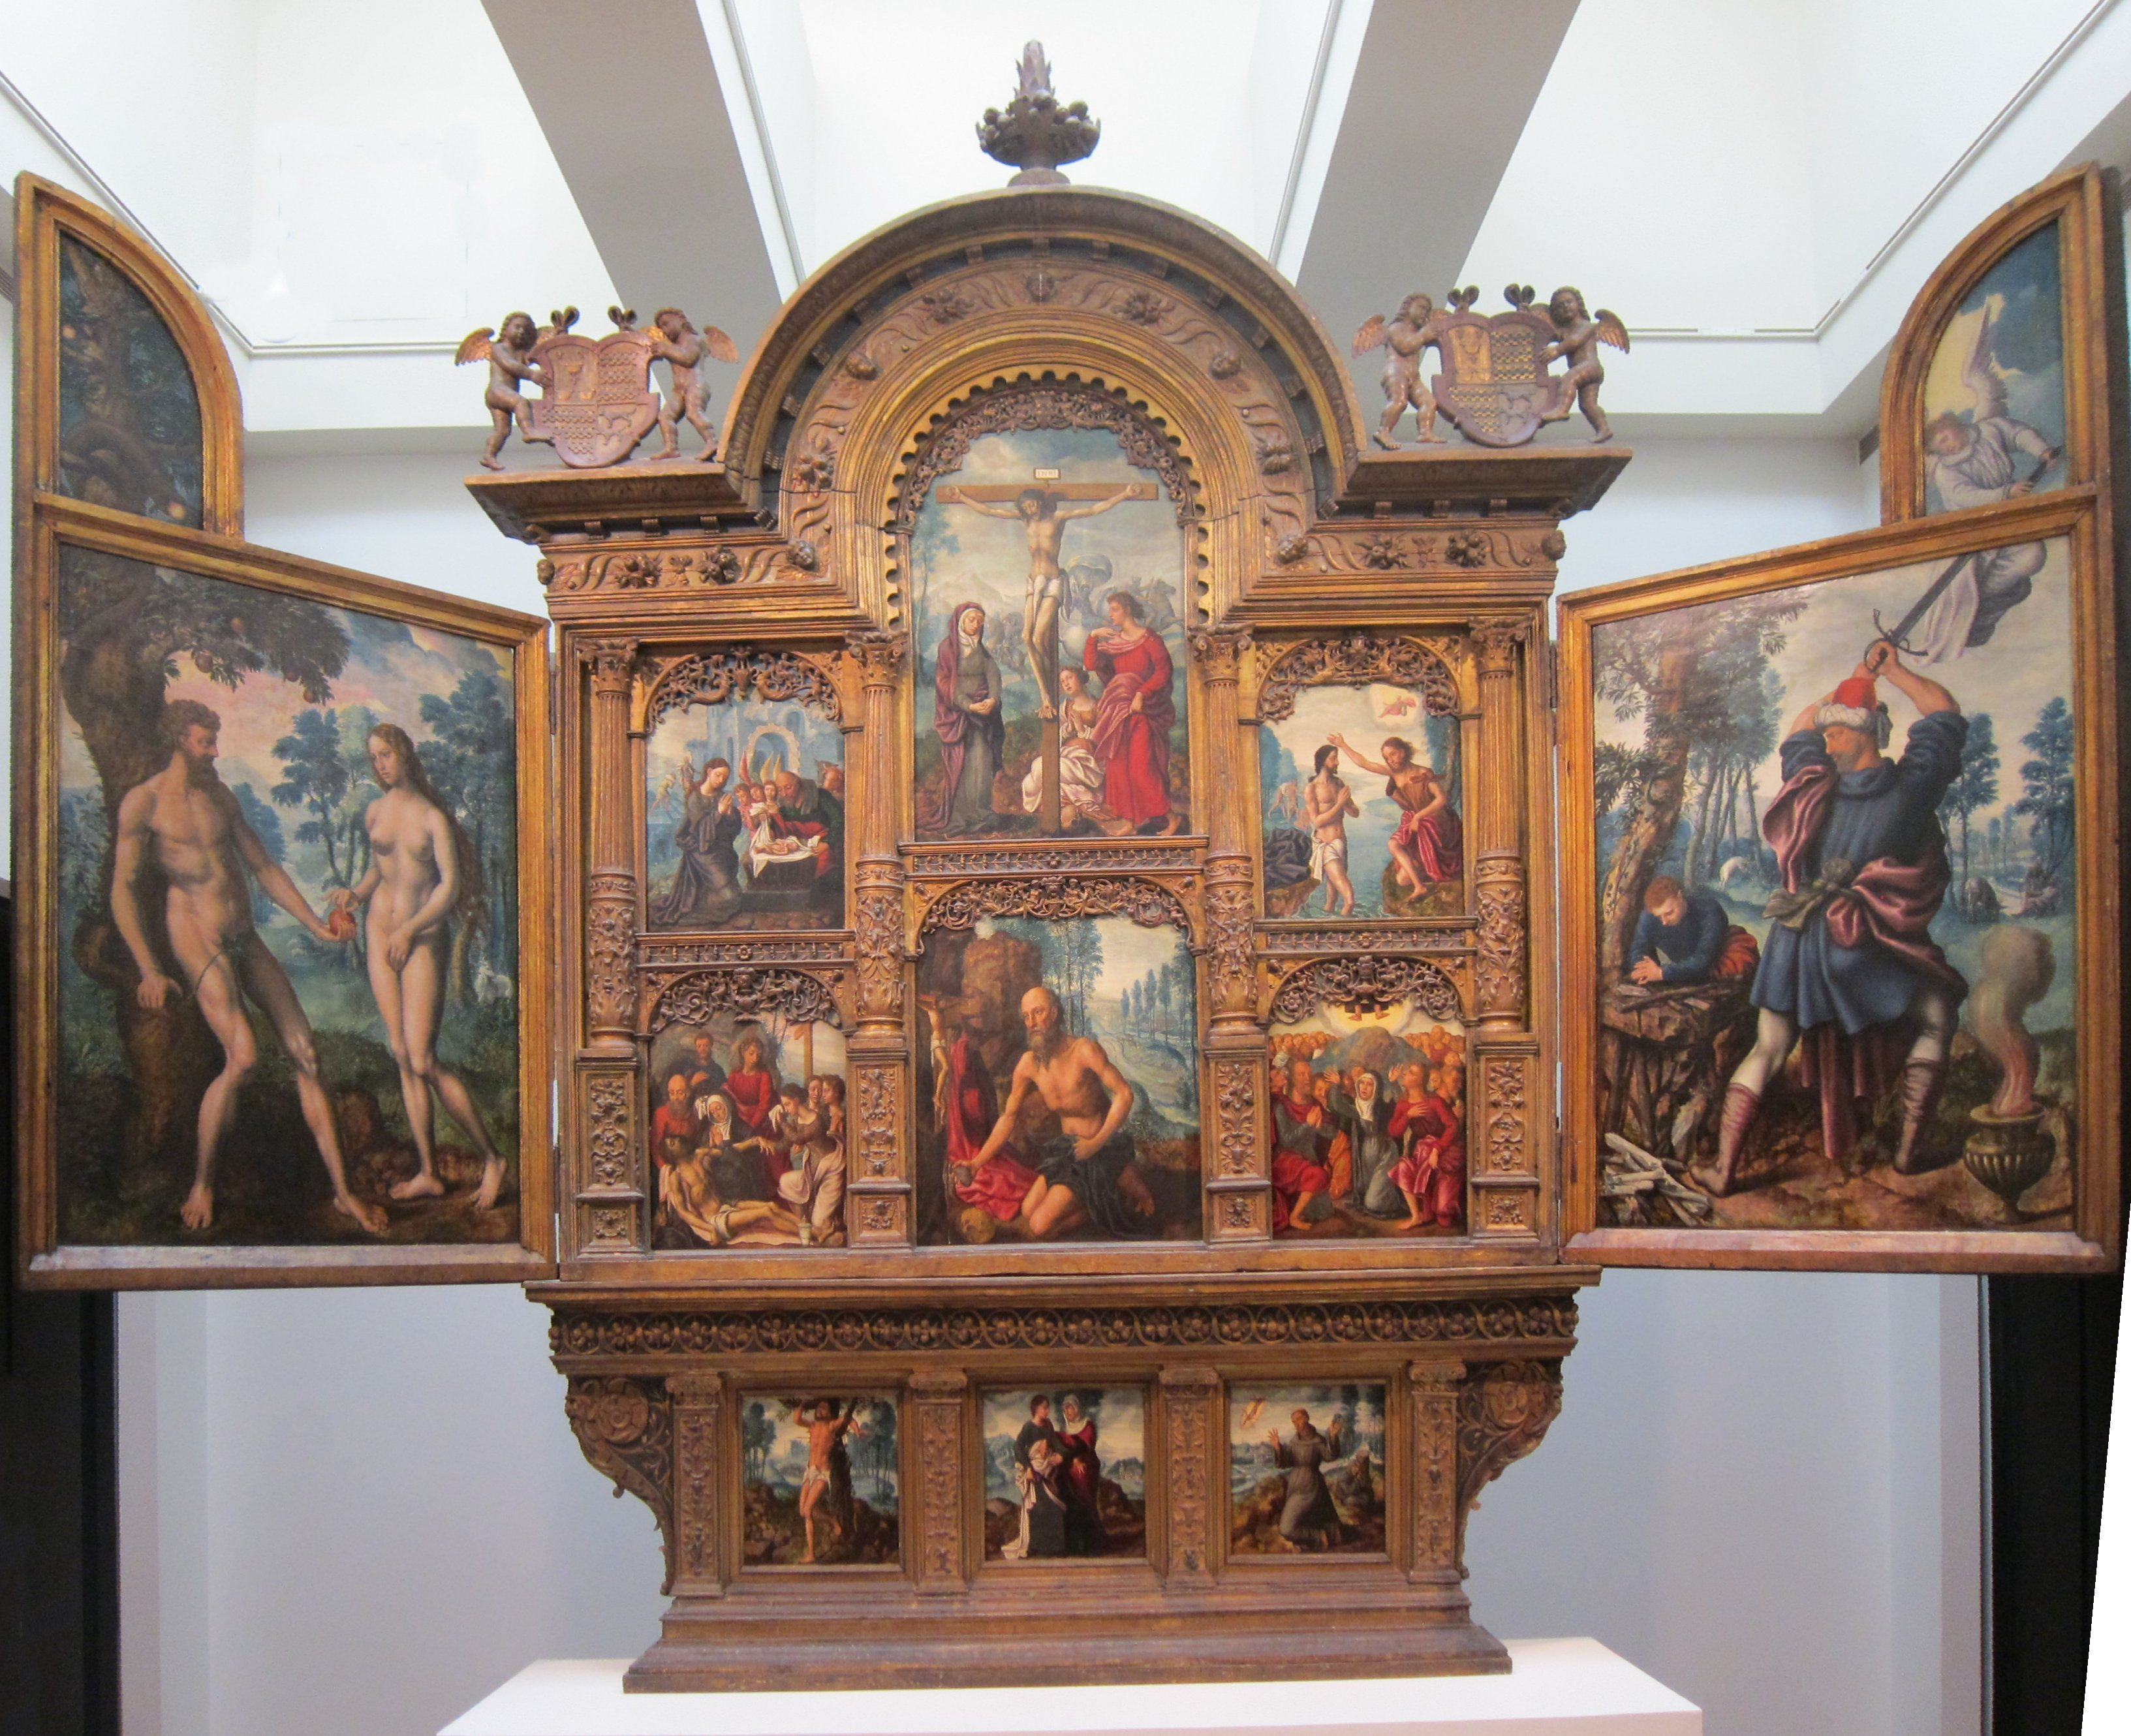
\includegraphics[width=0.75\linewidth]{retablo-de-tendilla}
	\caption{Retablo de Tendilla, Cincinnati Art Museum}
	\label{fig:wrapfig}
\end{figure}

Hacia finales del año 1558, tras la muerte de su protectora, la reina María de Hungría, la pareja volvió a Países Bajos, y se establecieron en su ciudad natal, Amberes. Ya en 1565, aún estando la pareja sin ningún hijo, Chrétien recibió una oferta para trabajar en 's-Hertogenbosch, por lo que decidieron mudarse allí. A partir de entonces, nada más se sabe de su vida, aparte de que (aunque no es completamente seguro) Catharina van Hemessen falleció por causas naturales en el año 1587, a los 60 años de edad.

\section{Reconocimiento}

A lo largo de su vida, van Hemessen fue mencionada en las respectivas obras de dos biógrafos italianos de artistas:
\begin{itemize}
	\item En la \textit{Descripción de los Países Bajos}\footnote{Del original, en italiano: \textit{Descrittione di Tutti i Paesi Bassi}}, de Lodovico Guicciardini, 1567.
	\item En las \textit{Vidas}\footnote{Del orig., en italiano: \textit{Le vite de' più eccellenti pittori, scultori, e architettori}}, de Giorgio Vasari, 1568.
\end{itemize}

Estas dos menciones implican que, en vida, Catharina van Hemessen gozó de éxito y una popularidad notorios dentro del mundo artístico, y es por ello que la reina María de Hungría confió en ella para formar parte de la corte y ser retratista allí. Esto se debe en gran parte a que su padre fue un artista de gran renombre, lo que es en parte negativo, dado que las pocas mujeres que llegaban a gozar de este reconocimiento no lo hacían por mérito propio, sino que eran otras personas cercanas ya conocidas las que influían en los pensamientos hacia dicha mujer, completamente ajenos a su capacidad artística real.

\section{Trabajo como pintora y retratista}

A pesar de que van Hemessen creó al menos dos obras de carácter religioso, ella era principalmente una retratista, creando la gran mayoría de sus obras como tal. Ocho retratos pequeños y dos pinturas de carácter religioso, todos datados entre 1548 y 1552, y con su firma inscrita han sobrevivido hasta nuestros días. Catharina retrató ostensiblemente a personas nobles y adineradas, tanto hombres como mujeres, normalmente frente a un fondo oscuro. Las figuras delicadas que pintaba eran de apariencia elegante y provistas de trajes y accesorios estilosos.\bigskip

Su obra más conocida es su \textit{Autorretrato}, mencionado anteriormente. Alrededor del mismo tiempo en que su \textit{Autorretrato} fue firmado (1548), Catharina van Hemessen pintó otra de sus obras más famosas: \textit{Joven dama} (1548), el cual podría ser un retrato de su hermana.\bigskip

Los retratos de van Hemessen se caracterizan por su realismo. Tanto su autorretrato como la media docena de retratos restante atribuidos a ella son obras pequeñas y calmadas. Los retratados, usualmente sentados, se representan frente a un fondo oscuro o neutro, y sus miradas rara vez se encuentran con los ojos del espectador.\bigskip

\chapter{Trabajos notables}

En este apartado se van a mostrar algunas de las obras más relevantes de Catharina van Hemessen, junto con alguna información cuando sea posible aportarla.

\section{\textit{Autorretrato}}

\textsc{Figura 3.1} (Galería de obras).\bigskip

Esta es posiblemente la obra más famosa de la artista flamenca. En ella se representa a la propia Catharina al comienzo de la creación de uno de sus retratos.
\begin{itemize}
	\item \textbf{Fecha}: 1548
	\item \textbf{Dimensiones}: 33x26,5 cm
	\item \textbf{Técnica}: pintura al óleo
	\item \textbf{Colección}: Kunstmuseum Basel, Basilea, Suiza
\end{itemize}

\section{\textit{Retrato de una dama}}

\textsc{Figura 3.2} (Galería de obras).\bigskip

A pesar de que no goza de tanta popularidad como la obra anterior, este es una de los más conocidos retratos de la artista flamenca. No se tiene constancia de quién es la mujer representada.
\begin{itemize}
	\item \textbf{Fecha}: ¿1551?
	\item \textbf{Dimensiones}: 22,9x17,8 cm
	\item \textbf{Técnica}: pintura al óleo sobre tabla de roble
	\item \textbf{Colección}: Fitzwilliam Museum, Londres, Reino Unido
\end{itemize}

\section{\textit{Retrato de un niño}}

\textsc{Figura 3.3} (Galería de obras).\bigskip

Esta obra no tiene un autor confirmado, pero se atribuye mayoritariamente a Catharina van Hemessen, principalmente por el estilo utilizado, y la naturaleza de las figuras. También podemos observar la presencia de un pequeño pájaro que se posa sobre la mano de un niño.
\begin{itemize}
	\item \textbf{Fecha}: 1559
	\item \textbf{Dimensiones}: 19,7x14,6 cm
	\item \textbf{Técnica}: pintura al óleo sobre tabla
	\item \textbf{Colección}: colección privada
\end{itemize}

\end{document}

%%%% REFERENCES %%%%
% https://en.wikipedia.org/wiki/Catharina_van_Hemessen
% http://jur.byu.edu/?p=5517
% https://www.ecured.cu/Caterina_van_Hemessen
% http://mujerespintoras.blogspot.com/2007/11/caterina-van-hemessen-1528-1587.html
% https://www.mujeresenlahistoria.com/2012/06/el-arte-flamenco-en-femenino-caterina.html
% https://www.abc.com.py/edicion-impresa/suplementos/cultural/caterina-van-hemessen-1528-1587-1486515.html
% http://sansemujeresenelrenacimiento.blogspot.com/p/caterina-van-hemessen.html
% https://en.wikipedia.org/wiki/List_of_paintings_by_Catharina_van_Hemessen

% SELF-PORTRAIT
%% https://www.hermitagemuseum.org/wps/portal/hermitage/digital-collection/01.%20Paintings/38355/!ut/p/z1/jZBNT8MwDIb_Cjv0SOx-pC27RUFijI1OEx8hF5RNXRvUJlUbVolfT0BcQFDmm6XHrx8bJAiQRh11pZy2RjW-f5Lpc8FYGsYclwWnl8iK7YZu-e0Vhgk8fgL4RzEEecr8BCCn45f_LfAXRP2aryuQnXL1uTYHCwJDcrZR2jhtqgFEnMeUehf5I-36JvNpd3RRFA884skXMO2jdy0Z9y1BQiOKYXyBmGdRluTphwwzuzj3Mn15KPuyJ6-9_3LtXDfMAwxwHEdSWVs1JdnbNsDfRmo7OBDfSejae_G2WuALbY4rNpu9A14z5fQ!/dz/d5/L2dBISEvZ0FBIS9nQSEh/?lng=en

% PORTRAIT OF A LADY
%% https://www.nationalgallery.org.uk/paintings/catharina-van-hemessen-portrait-of-a-woman
%% https://artuk.org/discover/artworks/portrait-of-a-lady-114862

% PORTRAIT OF A CHILD
%% https://arthistoryproject.com/artists/catharina-van-hemessen/portrait-of-a-child/
%% https://useum.org/artwork/Portrait-of-a-Child-Catharina-van-Hemessen